\documentclass[10pt,a4paper]{article}
\usepackage[utf8]{inputenc}
\usepackage[english]{babel}
\usepackage{amsmath}
\usepackage{amsfonts}
\usepackage{amssymb}
 \usepackage{cancel}
\usepackage{graphicx}

\title{Solid angle subtended by a tetrahedron computation}
\begin{document}

\maketitle


\includegraphics[scale=0.4]{tetra.png} 


\section{Notations}

Let

\begin{itemize}
	\item $\vec{a}$ be the vector $\vec{OA}$
	\item $\vec{b}$ be the vector $\vec{OB}$
	\item $\vec{c}$ be the vector $\vec{OC}$
	\item $a$ be the magnitude of the vector $\vec{OA}$
	\item $b$ be the magnitude of the vector $\vec{OB}$
	\item $c$ be the magnitude of the vector $\vec{OC}$
\end{itemize}

\section{Computation}

The solid angle $\Omega$ subtended by the triangular surface $ABC$ is:

$$
{\displaystyle \tan \left({\frac {1}{2}}\Omega \right)
  = {\frac {\left|{\vec {a}}\ {\vec {b}}\ {\vec {c}}\right|}
    {abc + \left({\vec {a}}\cdot {\vec {b}}\right)c
      + \left({\vec {a}}\cdot {\vec {c}}\right)b
      + \left({\vec {b}}\cdot {\vec {c}}\right)a}}}
$$

where $ \left|{\vec {a}}\ {\vec {b}}\ {\vec {c}}\right|={\vec {a}}\cdot ({\vec {b}}\times {\vec {c}}) $


\subsection{Numerator}


Given that $\vec{a} = \vec{OA} = \vec{OG} + \vec{GA}$ (and resp.
with $B$ and $C$), we get


\begin{align*}
\left|{\vec {a}}\ {\vec {b}}\ {\vec {c}}\right|
	& =  {\vec {a}} \cdot ({\vec {b}}\times {\vec {c}}) \\
	& =  {\vec {a}} \cdot ({(\vec{OG} + \vec{GB})} \times {(\vec{OG} + \vec{GC})}) \\
	& =  {(\vec{OG} + \vec{GA})} \cdot (\cancel{\vec{OG} \times \vec{OG}}
	                      + \vec{OG} \times \vec{GC}
	                      + \vec{GB} \times \vec{OG}
	                      + \vec{GB} \times \vec{GC}) \\
	& = \cancel{\vec{OG} \cdot (\vec{OG} \times \vec{GC})}
	                      + \cancel{\vec{OG} \cdot (\vec{GB} \times \vec{OG})}\\
         & + \vec{OG} \cdot (\vec{GB} \times \vec{GC})
	  + \vec{GA} \cdot (\vec{OG} \times \vec{GC})
	  + \vec{GA} \cdot (\vec{GB} \times \vec{OG})
	  + \cancel{\vec{GA} \cdot (\vec{GB} \times \vec{GC})} \\
	& = \vec{OG} \cdot (\vec{GB} \times \vec{GC})
	+ \vec{OG} \cdot (\vec{GC} \times \vec{GA})
	+ \vec{OG} \cdot (\vec{GA} \times \vec{GB}) \\
	& = \vec{OG} \cdot (\vec{GB} \times \vec{GC})
	+ \vec{OG} \cdot (\vec{GC} \times \vec{GA})
	+ \vec{OG} \cdot (\vec{GA} \times \vec{GB})\\
	& = \vec{OG} \cdot \left(\vec{GB} \times \vec{GC}
	+\vec{GC} \times \vec{GA}
	+ \vec{GA} \times \vec{GB} \right)
\end{align*}

since $G$ is the centroid of $ABC$, 

\begin{equation}
\vec{GA} + \vec{GB} + \vec{GC}= 0
\label{eq1}
\end{equation}. We obtain

\begin{align}
\left|{\vec {a}}\ {\vec {b}}\ {\vec {c}}\right|
& = \vec{OG} \cdot \left(\vec{GB} \times \vec{GC}
	+\vec{GC} \times \vec{GA}
	+ \vec{GA} \times \vec{GB} \right) \nonumber \\
& = \vec{OG} \cdot \left(\vec{GB} \times \vec{GC}
	+\vec{GC} \times (-\vec{GB} - \vec{GC})
	+ (-\vec{GB} - \vec{GC}) \times \vec{GB} \right) \nonumber \\
& = \vec{OG} \cdot \left(\vec{GB} \times \vec{GC}
	+\vec{GC} \times (-\vec{GB}) + \cancel{\vec{GC} \times (- \vec{GC})}
	+ \cancel{(-\vec{GB}) \times \vec{GB}} + (- \vec{GC}) \times \vec{GB} \right) \nonumber \\
& = \vec{OG} \cdot \left(3 \vec{GB} \times \vec{GC} \right) \nonumber \\
& = 3 \vec{OG} \cdot \left( \vec{GB} \times \vec{GC} \right)
\end{align}

\subsection{Denominator}


First let's see the term in $c$
\begin{align*}
 \left({\vec {a}}\cdot {\vec {b}}\right)c 
	=& \left( \vec{OG} + \vec{GA} \right) \cdot \left( \vec{OG} + \vec{GB} \right) c \\
	 =& (g^2 +  \vec{OG} \cdot \vec{GB}	+ \vec{GA} \cdot \vec{OG} + \vec{GA} \cdot \vec{GB}    ) c
\end{align*}

Using \eqref{eq1}

\begin{align}
 \left({\vec {a}}\cdot {\vec {b}}\right)c 
	 =& (g^2 +  \vec{OG} \cdot \vec{GB}	+ (-\vec{GB} - \vec{GC}) \cdot \vec{OG} + (-\vec{GB} - \vec{GC}) \cdot \vec{GB}    ) c \nonumber \\
	 =& (g^2 - ||GB||^2 - \vec{OG} \cdot \vec{GC} - \vec{GC} \cdot \vec{GB})c
\end{align}



Now, the term in $b$


\begin{align*}
 \left({\vec {a}}\cdot {\vec {c}}\right)c 
	=& \left( \vec{OG} + \vec{GA} \right) \cdot \left( \vec{OG} + \vec{GC} \right) b \\
	 =& (g^2 +  \vec{OG} \cdot \vec{GC}	+ \vec{GA} \cdot \vec{OG} + \vec{GA} \cdot \vec{GC}    ) b
\end{align*}

Using \eqref{eq1}

\begin{align}
 \left({\vec {a}}\cdot {\vec {c}}\right)b
	 =& (g^2 +  \vec{OG} \cdot \vec{GC}	+ (-\vec{GB} - \vec{GC}) \cdot \vec{OG} + (-\vec{GB} - \vec{GC}) \cdot \vec{GC}    ) b \nonumber \\
	 =& (g^2 - ||GC||^2 - \vec{OG} \cdot \vec{GC} - \vec{GC} \cdot \vec{GB})b
\end{align}


For the third term there is no simplification

\begin{align}
 \left({\vec {b}}\cdot {\vec {c}}\right)a 
	=& \left( \vec{OG} + \vec{GB} \right) \cdot \left( \vec{OG} + \vec{GC} \right) a
\end{align}


For the computation of the norms, we can use:

\begin{align*}
a^2 &= ||OG||^2 + ||GA||^2\\
    &=  g^2 + ||GA||^2
\end{align*}

thus

\begin{align}
g^2 &= a^2 - ||GA||^2 \nonumber \\ 
    &= b^2 - ||GB||^2 \nonumber \\
    &= c^2 - ||GC||^2
\end{align}

and

\begin{align}
(abc)^2 &= (g^2 + ||GA||)^2(g^2 + ||GB||)^2(g^2 + ||GC||)^2 
\end{align}

\end{document}
